\documentclass{article}
\usepackage{float}
\usepackage[pdftex]{graphicx}
\usepackage{listings}
\usepackage{xcolor}
\lstset{basicstyle=\ttfamily,
  showstringspaces=false,
  commentstyle=\color{red},
  keywordstyle=\color{blue}
}
\begin{document}

\author{Jon Robison}
\title{CS595 Assignment 5}
\maketitle

Q1.  Determine if the friendship paradox holds for your Facebook account.\\
Create a graph of the number of friends (y-axis) and the friends sorted\\
by number of friends (x-axis).  (The friends don't need to be labeled \\
on the x-axis.)  Do include yourself in the graph and label yourself\\
accordingly.\\
Compute the mean, standard deviation, and median of the number of friends\\
that your friends have. \\*

From a sample size of 272, 9 do not share friend count data publicly and\\
20 have other privacy restrictions precluding calculation.\\
See Appendix A for translator\\
Average: 639.065843621 \\
Std deviation: 465.913488086 \\
Median: 535.0 \\
\graphicspath{{q1/}}
\begin{figure}[H]
  \centering
  \caption{Facebook Friend Count}
  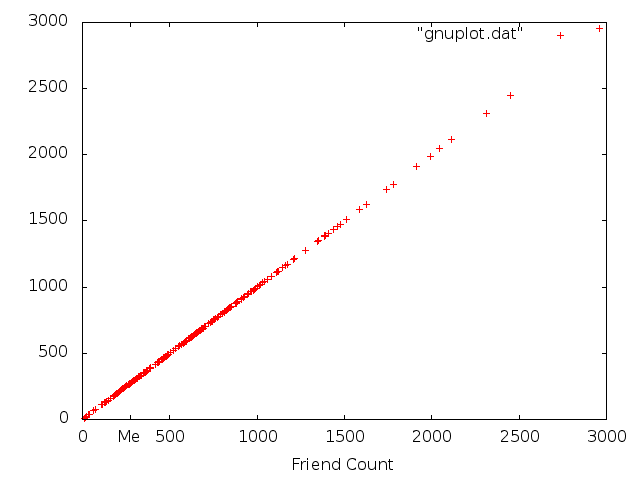
\includegraphics[scale=.42]{scatter.png}
\end{figure}
\clearpage

Q2. Determine if the friendship paradox holds for your Twitter account.\\
Since Twitter is a directed graph, use ``followers'' as value you measure\\
(i.e., ``do your followers have more followers than you?'').\\
\\
Generate the same graph as in question 1, and calcuate the same \\
mean, standard deviation, and median values.\\*

See Appendix B for program\\
Average: 521.293532338\\
Std deviation: 1264.46308524\\
Median: 197.0\\
\graphicspath{{q2/}}
\begin{figure}[H]
  \centering
  \caption{Twitter Friend Count}
  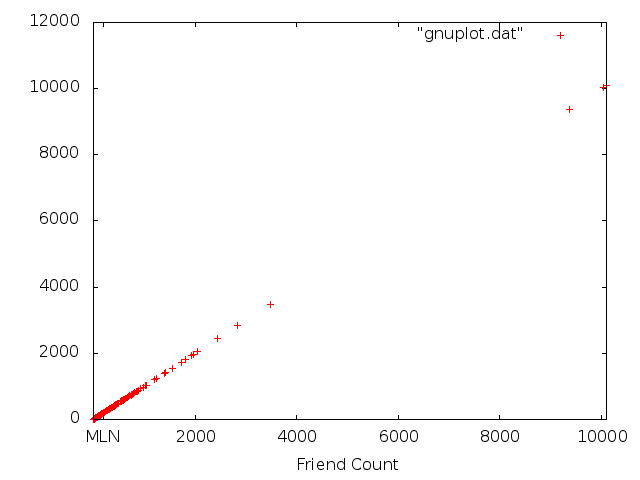
\includegraphics[scale=.45]{scatter.png}
\end{figure}
\clearpage

Q3 EC. Repeat question 1, but with your LinkedIn profile\\
\\*

Q4 EC. Repeat question 2, but change ``followers'' to ``following''?  In\\
other words, are the people I am following following more people?\\
\\*

\appendix
\newpage
Appendix A
\lstinputlisting[language=python]{q1/createPlot.py}

\newpage
Appendix B
\lstinputlisting[language=python]{q2/twitterFriendCounter.py}

\end{document} 
